\documentclass[conference]{IEEEtran}
\IEEEoverridecommandlockouts
\usepackage{cite}
\usepackage{amsmath,amssymb}
\usepackage{graphicx}
\usepackage{booktabs}
\usepackage{array}
\usepackage[hyphens]{url}
\graphicspath{{figures/}}

\begin{document}

\title{Reading Garments from Unlabelled Product Photos: Outline, Multi-Colour Palette and Two-Level Design Regions for Sewing-Pattern-Driven Virtual Try-On}

\author{\IEEEauthorblockN{Saumy Bhargava, Tanuj}
\IEEEauthorblockA{Department of CSE\\
CO CSC 601 Computer Vision, Course Project}}

\maketitle

\begin{abstract}
Virtual try-on systems that simulate a garment on a measured body need more than a single product photo: they need the garment's outline, all of its colours, every printed design with its type, and the knowledge of which photo shows the front and which the back. We rebuild the photo-reading stage of such a pipeline and, at every stage, compare classical computer-vision methods with pretrained models used zero-shot and with small models trained for this work. The final pipeline (i) assigns front, back, side and other views to a set of unlabelled photos with a trained classifier and a joint set-level decision, (ii) segments the garment with a clothes-parser box that prompts SAM~2, plus a simple scene rule that keeps both halves of colour-block tops, (iii) extracts a multi-colour palette with a colour region map by mean shift in CIELAB, (iv) outlines each design region inside the garment and labels it as text, graphic, logo, stripes, colour block or pattern, and (v) builds one texture per sewing-pattern panel by thin-plate-spline warping. The scoring metrics were chosen by controlled damage tests and checked against a blind ranking by eye (Kendall $\tau_b$ 0.72--0.83). End to end on five real product photos the pipeline score rises from 0.407 to 0.960; on public datasets with exact labels the mean garment IoU rises from 0.756 to 0.892, and the correct front is chosen in 85.4\,\% of shuffled photo sets.
\end{abstract}

\begin{IEEEkeywords}
garment segmentation, colour extraction, design region detection, view classification, SAM 2, virtual try-on, sewing patterns
\end{IEEEkeywords}

\section{Introduction}
Sewing-pattern-driven 3D fashion design builds a garment from 2D panels and simulates it on a body~\cite{luo2026survey}. Parametric pattern construction works best when garment measurements and appearance are read automatically from images~\cite{lyu2026review}, and virtual fitting rooms depend on a reliable garment asset pipeline~\cite{cannavo2024pipeline}. Measurement-conditioned try-on~\cite{nikolaev2026quantfit} and parsing-based try-on~\cite{kim2025capvton} both assume that the garment has already been separated cleanly from skin and background.

This paper studies the \emph{product ingestion} stage of such a system: given one or several product photos of a T-shirt, produce (1) the view of each photo, (2) the garment outline, (3) its shape, (4) all of its colours, (5) every design region with its type, and (6) one texture image per sewing-pattern panel. The existing stage (called v0 below) used a single photo, a SAM~2 centre-point prompt, K-means colour clustering with an HSV skin filter, and a Canny-plus-FFT design detector. On five real product photos it scored 0.407 out of 1, and seven concrete bugs were reproduced (Section~\ref{sec:baseline}).

The contributions are:
\begin{itemize}
\item A scoring framework whose metrics were selected by controlled damage tests and validated against a blind ranking by eye.
\item A multi-photo view assignment that combines a trained classifier with a joint front/back decision and a same-garment check.
\item A segmentation chain (parser box $\rightarrow$ SAM~2) with a head-visibility rule that fixes colour-block tops without loss elsewhere, compared with 58 classical, zero-shot and trained variants, including a YOLO26s-seg model fine-tuned here.
\item Multi-colour extraction that never reduces a garment to one colour, and two-level outlining of design regions with zero-shot relabelling.
\item A systematic comparison of syllabus methods (filters, edge and corner detectors, graph cut, clustering, Gabor/wavelet texture, classical classifiers) with modern models at every stage, keeping every failed attempt.
\end{itemize}

\section{Related Work}
\textbf{Promptable and semantic segmentation.} SAM~2~\cite{ravi2024sam2} segments any object from point or box prompts; SegFormer~\cite{xie2021segformer} provides efficient semantic segmentation and is available with clothes-parsing weights. Open-vocabulary detectors such as Grounding DINO~\cite{liu2024groundingdino} and the YOLO family~\cite{ultralytics} supply boxes or masks from text or fixed classes. Classical alternatives include graph-cut segmentation (GrabCut)~\cite{rother2004grabcut} and mean shift~\cite{comaniciu2002meanshift}.

\textbf{Vision-language features.} CLIP~\cite{radford2021clip} and SigLIP~2~\cite{tschannen2025siglip2} give image embeddings usable zero-shot or as frozen features for small classifiers; Marqo-FashionSigLIP~\cite{marqo2024fashionsiglip} adapts them to fashion.

\textbf{Fashion datasets.} Fashionpedia~\cite{jia2020fashionpedia} provides garment masks and fine-grained attributes, VITON-HD~\cite{choi2021vitonhd} product and person photos with garment masks, DeepFashion In-shop~\cite{liu2016deepfashion} several views per item, and Fashion Product Images~\cite{aggarwal2019fpi} colour labels. Text in images is found by the CRAFT detector used in EasyOCR~\cite{baek2019craft}. Body and garment measurement from images is reviewed in~\cite{mohammedkhan2025review}.

\section{Method}
Table~\ref{tab:pipeline} summarises each stage before and after this work and the methods compared. Every new default keeps the old method selectable.

\begin{table*}[t]
\caption{Pipeline stages: the original method (v0), the final default and the methods compared}
\label{tab:pipeline}
\centering
\footnotesize
\begin{tabular}{@{}p{2.1cm}p{4.0cm}p{5.3cm}p{5.4cm}@{}}
\toprule
Stage & v0 & Final default & Methods compared \\
\midrule
Views (several photos) & CLIP zero-shot (never loaded); first photo used & SigLIP~2 features + logistic regression trained on In-shop view labels; joint front/back choice; same-garment check & Naive Bayes, KNN, MLP, logistic regression, $\pm$PCA/LDA; face cues; CLIP, FashionSigLIP zero-shot \\
Outline & SAM~2 centre point; corner flood fill & \texttt{v1\_auto}: SegFormer parser box + interior point $\rightarrow$ SAM~2; ``Skirt'' class added only when no head is visible & GrabCut, K-means, mean shift, region growing, MRF; YOLO, YOLOE, Grounding DINO, RMBG; votes; 14 selection rules; fine-tuned YOLO26s-seg \\
Filtering & Gaussian + auto-Canny & Bilateral + Laplacian zero crossings for print edges; no global enhancement before colour & HE, CLAHE, gamma, grey-world, Retinex, homomorphic; mean/median/Gaussian/bilateral; Sobel, Prewitt, Scharr, Laplacian, LoG, DoG, Canny; pyramids \\
Colour & K-means; HSV skin filter; one base colour & Mean shift in CIELAB, merge within $\Delta E_{00}<5$, guarded skin removal; palette with roles and colour region map & K-means, K-medoids, GMM (BIC), mean shift \\
Designs & Canny contours + global FFT test; one box & Level 1 garment, level 2 typed regions (\texttt{v4\_relabel}): colour deviation, OCR, Hough stripes, colour blocks, cleaned Grounding DINO boxes; SigLIP~2 relabelling; fixed periodicity test & Canny, Gabor bank, DWT texture, Hough, FFT; SAM~2, Grounding DINO, OCR \\
Shape & fixed ratios & Landmarks from the outline (convexity defects, curvature); sleeve class; width/length ratios & Harris, Shi-Tomasi, Hessian, FAST, ORB, SIFT, AKAZE \\
Attributes & none & Pattern, sleeve, neckline classifiers on frozen SigLIP~2 features (Fashionpedia) & Naive Bayes, KNN, MLP, LR, LDA, PCA, self-training \\
Panel textures & one box homography into the front panel; flat back & Torso/sleeve split; thin-plate-spline warp per panel; back from the back photo & Homography, affine, TPS \\
\bottomrule
\end{tabular}
\end{table*}

\subsection{View assignment from several unlabelled photos}
Each photo is embedded with frozen SigLIP~2~\cite{tschannen2025siglip2} features, and a logistic-regression classifier trained on the view labels encoded in DeepFashion In-shop~\cite{liu2016deepfashion} file names predicts front, back, side or other. Naive Bayes, KNN, an MLP and LDA~\cite{fisher1936lda} on PCA-reduced features were compared. Instead of deciding photo by photo, the front and back are chosen jointly over the set (they must be different photos and maximise the joint probability). A same-garment check (feature cosine similarity plus a colour histogram distance, grouped by correlation clustering) flags photos of a different item.

\subsection{Garment outline}
The SAM~2~\cite{ravi2024sam2} centre-point prompt of v0 often returned only the print or a leaking region. In the final chain (\texttt{v1}), a SegFormer clothes parser~\cite{xie2021segformer} yields an upper-clothes region whose bounding box and an interior point prompt SAM~2 for a single mask. Holes are filled from a padded border, and the outline is a Douglas--Peucker~\cite{douglas1973} polygon of the mask contour. The parser labels the lower half of a colour-block top as ``Skirt''. Including that class always (\texttt{v1\_all}) fixes such tops but harms photos of people. We therefore use a scene rule (\texttt{v1\_auto}):
\begin{equation}
\text{use Skirt} \iff A_{\text{skirt}} \geq 1\,\% \;\wedge\; A_{\text{face}} + A_{\text{hair}} < 1\,\%,
\end{equation}
where $A$ is the share of image pixels per parser class: with no head visible, the photo is a flat product shot or a torso crop, so the ``skirt'' is the top's own lower half. The rule reuses the parser output and adds no model pass. It was selected from 14 candidate rules (model confidence, edge alignment, skirt geometry, extra prompts) designed on 405 public images and checked on 400 held-out images.

We also fine-tuned YOLO26s-seg~\cite{ultralytics} on 1,468 garment masks from VITON-HD and Fashionpedia (about 30 minutes on a 6\,GB GPU) as a trained alternative.

\subsection{Multi-colour extraction}
Pixels inside the garment mask are converted to CIELAB and clustered by mean shift~\cite{comaniciu2002meanshift}; clusters closer than $\Delta E_{00}=5$~\cite{sharma2005ciede2000} are merged as shades of one fabric. Skin is removed only by the parser's skin labels when a person is present, instead of the wide HSV range that deleted pink, tan and brown fabric. The output is a palette (every major colour with its share and a fabric or print role) and a colour region map, so a colour-block shirt keeps both blocks. K-means, K-medoids~\cite{kaufman1990} and Gaussian mixtures selected by BIC were compared.

\subsection{Two-level design regions}
Level 1 is the garment outline. Level 2 finds every design region inside it, ignoring a band along the outline. Proposals come from colour deviation from the fabric colour, OCR text boxes~\cite{baek2019craft}, Hough~\cite{duda1972hough} line families for stripes, colour blocks from the palette, and Grounding DINO~\cite{liu2024groundingdino} boxes cleaned by size and overlap. Each region is retyped zero-shot by SigLIP~2 with prompt ensembles; a ``plain fabric'' verdict removes it. Text inside a graphic is kept as part of it, and a small second text line is split off by glyph height. The periodicity (all-over pattern) test was rebuilt: a windowed FFT of an inner patch, peaks measured against the radially averaged spectrum, and mirrored peak pairs required. Gabor filter banks~\cite{jain1991gabor} and wavelet~\cite{mallat1989} texture segmentation, Canny~\cite{canny1986} contours and SAM~2 automatic masks were also compared.

\subsection{Shape, attributes and panel textures}
Landmarks (armpits from convexity defects, shoulders, cuffs and hem from contour curvature) give the sleeve class and width/length ratios; nine corner and keypoint detectors, including Harris~\cite{harris1988}, Shi--Tomasi~\cite{shi1994}, ORB~\cite{rublee2011orb} and SIFT~\cite{lowe2004sift}, were compared as landmark sources. Small classifiers on frozen SigLIP~2 features trained on Fashionpedia~\cite{jia2020fashionpedia} predict textile pattern, sleeve length and neckline. Finally, the torso and each sleeve are warped onto their sewing-pattern panels with thin-plate splines~\cite{bookstein1989tps} fitted to landmark correspondences, replacing a single box-to-box homography; the back panel is taken from the back photo when one exists.

\section{Evaluation Protocol}
\label{sec:baseline}
\subsection{Data}
Five real product photos from the Mirra catalogue (three worn, two flat; one back view; one white/teal colour-block top) were labelled by hand: garment mask, palette, design boxes with types, and view. These references are approximate, and four masks were started from SAM~2 candidates, which favours SAM~2-based methods; headline outline numbers therefore come from public data with exact masks: VITON-HD product and person photos~\cite{choi2021vitonhd} and Fashionpedia street photos~\cite{jia2020fashionpedia}. Views were evaluated on DeepFashion In-shop~\cite{liu2016deepfashion} test items and colour names on Fashion Product Images~\cite{aggarwal2019fpi}.

On the five photos, v0 showed seven reproducible bugs: the HSV skin filter deleted warm fabrics; white and black were never chosen as base colour; a flat colour crashed K-means; the FFT pattern test fired on every image; the corner flood fill turned masks touching the corner into the full image; and two quality signals were constant.

\subsection{Metrics and their validation}
Candidate metrics were applied to deliberately damaged references (grown borders, leak blobs, missing chunks, colour shifts, a dropped colour block, dropped or retyped design boxes). IoU barely reacts to a border grown by 1\,\% of the diagonal (0.928), the 95th-percentile Hausdorff distance is not monotonic, the base-colour error ignores a lost colour block ($\Delta E$ 0.40), and box F1 ignores wrong types. The chosen area scores are
\begin{align}
S_{\text{out}} &= \tfrac{1}{2}\left(\text{IoU} + F_{b}^{1\%}\right),\\
S_{\text{col}} &= \max\!\left(0,\, 1 - \overline{\Delta E}_{\text{pal}}/30\right),\\
S_{\text{des}} &= \tfrac{1}{3}\left(F1_{@0.3} + \text{IoU}_{\text{pix}} + \text{Acc}_{\text{type}}\right),
\end{align}
where $F_b^{1\%}$ is the boundary F-score at a tolerance of 1\,\% of the image diagonal and $\overline{\Delta E}_{\text{pal}}$ is the share-weighted CIEDE2000 distance between matched palette colours. The view score is the share of correct views, and the pipeline score is the mean of the four.

To check agreement with human judgement, eight segmentation methods were drawn on each photo under hidden letters, ranked by eye before the key was opened, and compared with each metric's ranking using Kendall's $\tau_b$~\cite{kendall1938}. All metrics agreed strongly: IoU 0.833, outline score 0.766, HD95 0.751, boundary F 0.719. The outline score is kept as headline because the damage tests show border errors that IoU misses.

\section{Results}

\subsection{End to end}
Table~\ref{tab:e2e} and Fig.~\ref{fig:beforeafter} give the scores of the full pipeline on the five photos. The first integrated pipeline already lifts the score from 0.407 to 0.911; two improvement passes (\texttt{v1\_auto} segmentation and \texttt{v4\_relabel} designs) reach 0.960. Mask IoU is 0.982 (colour-block top: 0.562 $\rightarrow$ 0.939), the palette error is $\Delta E_{00}$ 1.13 and the colour-block top's base colour error drops from 67.7 to 1.08. Design F1 is 0.848, no design is reported on the plain shirt, and type accuracy is 1.0.

\begin{table}[t]
\caption{End-to-end scores on the five product photos}
\label{tab:e2e}
\centering
\begin{tabular}{@{}lccc@{}}
\toprule
Area & v0 & First pipeline & Final \\
\midrule
Outline & 0.658 & 0.919 & \textbf{0.974} \\
Colour & 0.808 & 0.951 & \textbf{0.962} \\
Design & 0.160 & 0.774 & \textbf{0.903} \\
View & 0.000 & 1.000 & \textbf{1.000} \\
\midrule
Pipeline & 0.407 & 0.911 & \textbf{0.960} \\
\bottomrule
\end{tabular}
\end{table}

\begin{figure}[t]
\centering
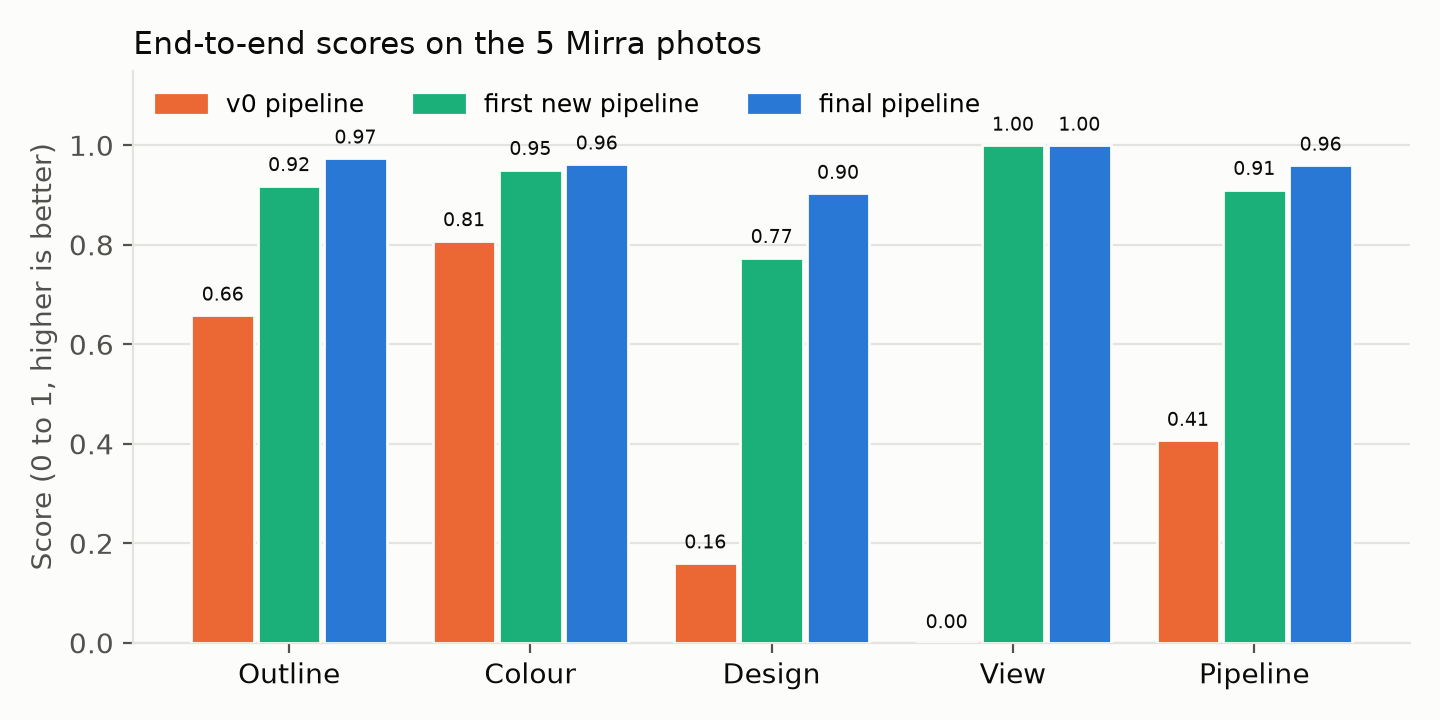
\includegraphics[width=\columnwidth,height=0.3\textheight,keepaspectratio]{fig_before_after_scores.png}
\caption{Per-area scores of v0, the first integrated pipeline and the final pipeline on the five product photos.}
\label{fig:beforeafter}
\end{figure}

\subsection{Garment outline}
Table~\ref{tab:outline} and Fig.~\ref{fig:outlinepublic} compare outline methods on public images with exact masks. Replacing the centre-point prompt with a parser box raises IoU on photos of people by 0.118 (95\,\% CI 0.082--0.156) and on street photos by 0.277 (0.213--0.342), with product photos unchanged. The best classical method, GrabCut, reaches 0.618 and zero-shot YOLO variants 0.64--0.75. Majority votes of two or three models did not help. \texttt{v1\_auto} improves on \texttt{v1} on 400 held-out images (0.8966 vs.\ 0.8940; pooled gain $+0.0027$, CI $+0.0005$ to $+0.0059$); it fires only on flat product photos and never lowers person or street results. The fine-tuned YOLO26s-seg matches \texttt{v1} (0.889) at 5\,\% of its run time but is weaker on street photos and misses the teal half of the colour-block top, so it is kept as a comparison. Fig.~\ref{fig:sam2} shows why the v0 prompt failed: SAM~2's most confident candidate is the print, not the shirt.

\begin{table}[t]
\caption{Garment IoU on public data with exact masks}
\label{tab:outline}
\centering
\footnotesize
\setlength{\tabcolsep}{3pt}
\begin{tabular}{@{}lcccccc@{}}
\toprule
Method & Prod. & Person & Street & Macro & Fail & s/img \\
\midrule
v0 (SAM~2 centre pt.) & 0.932 & 0.775 & 0.562 & 0.756 & 8.0\% & 0.55 \\
GrabCut (classical) & -- & -- & -- & 0.618 & -- & -- \\
YOLOE zero-shot & -- & -- & -- & 0.641 & 26.6\% & 0.30 \\
YOLO person $-$ skin & -- & -- & -- & 0.751 & 12.7\% & 0.13 \\
v1 (parser box $\rightarrow$ SAM~2) & 0.936 & 0.893 & 0.838 & 0.889 & 1.1\% & 0.59 \\
\textbf{v1\_auto (final)} & 0.944 & 0.893 & 0.838 & \textbf{0.892} & 1.1\% & 0.59 \\
YOLO26s-seg (fine-tuned) & 0.979 & 0.901 & 0.788 & 0.889 & 1.8\% & 0.03 \\
\bottomrule
\end{tabular}
\end{table}

\begin{figure}[t]
\centering
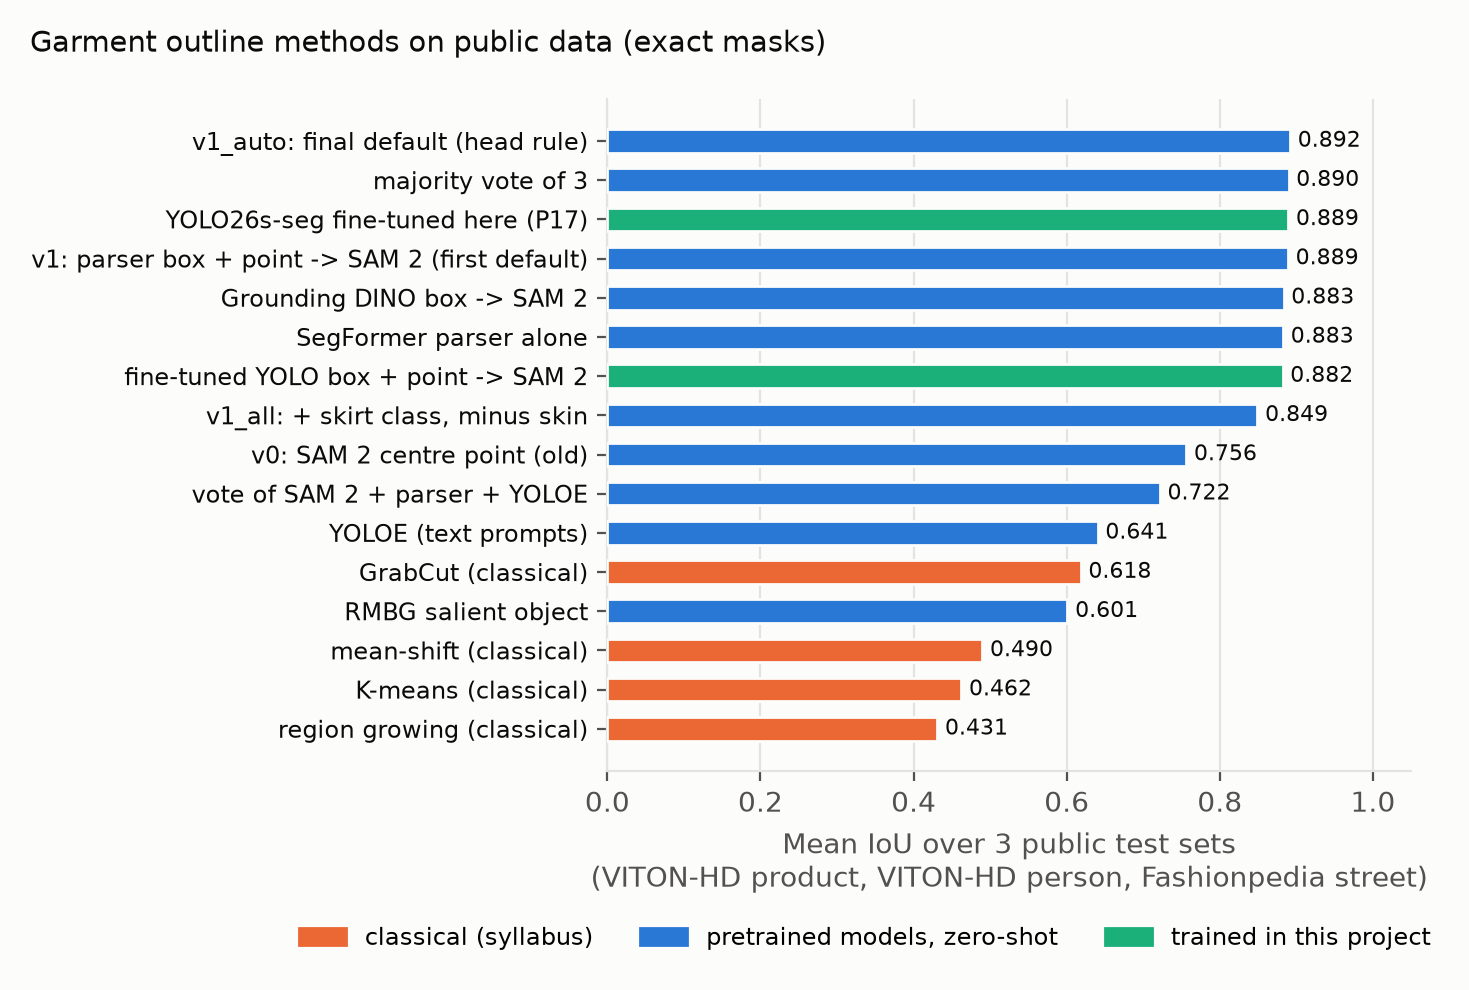
\includegraphics[width=\columnwidth,height=0.32\textheight,keepaspectratio]{fig_outline_public_iou.png}
\caption{Mean garment IoU of outline methods on public data, by family: classical (syllabus), pretrained zero-shot, and trained in this work.}
\label{fig:outlinepublic}
\end{figure}

\begin{figure}[t]
\centering
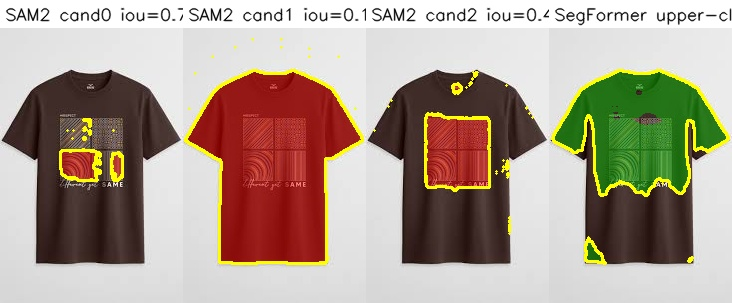
\includegraphics[width=\columnwidth,height=0.22\textheight,keepaspectratio]{p00_sam2_candidates_c_004.jpg}
\caption{The three SAM~2 candidates for a centre-point prompt on a flat shirt: the highest-scoring candidate covers only the printed square.}
\label{fig:sam2}
\end{figure}

\begin{figure*}[t]
\centering
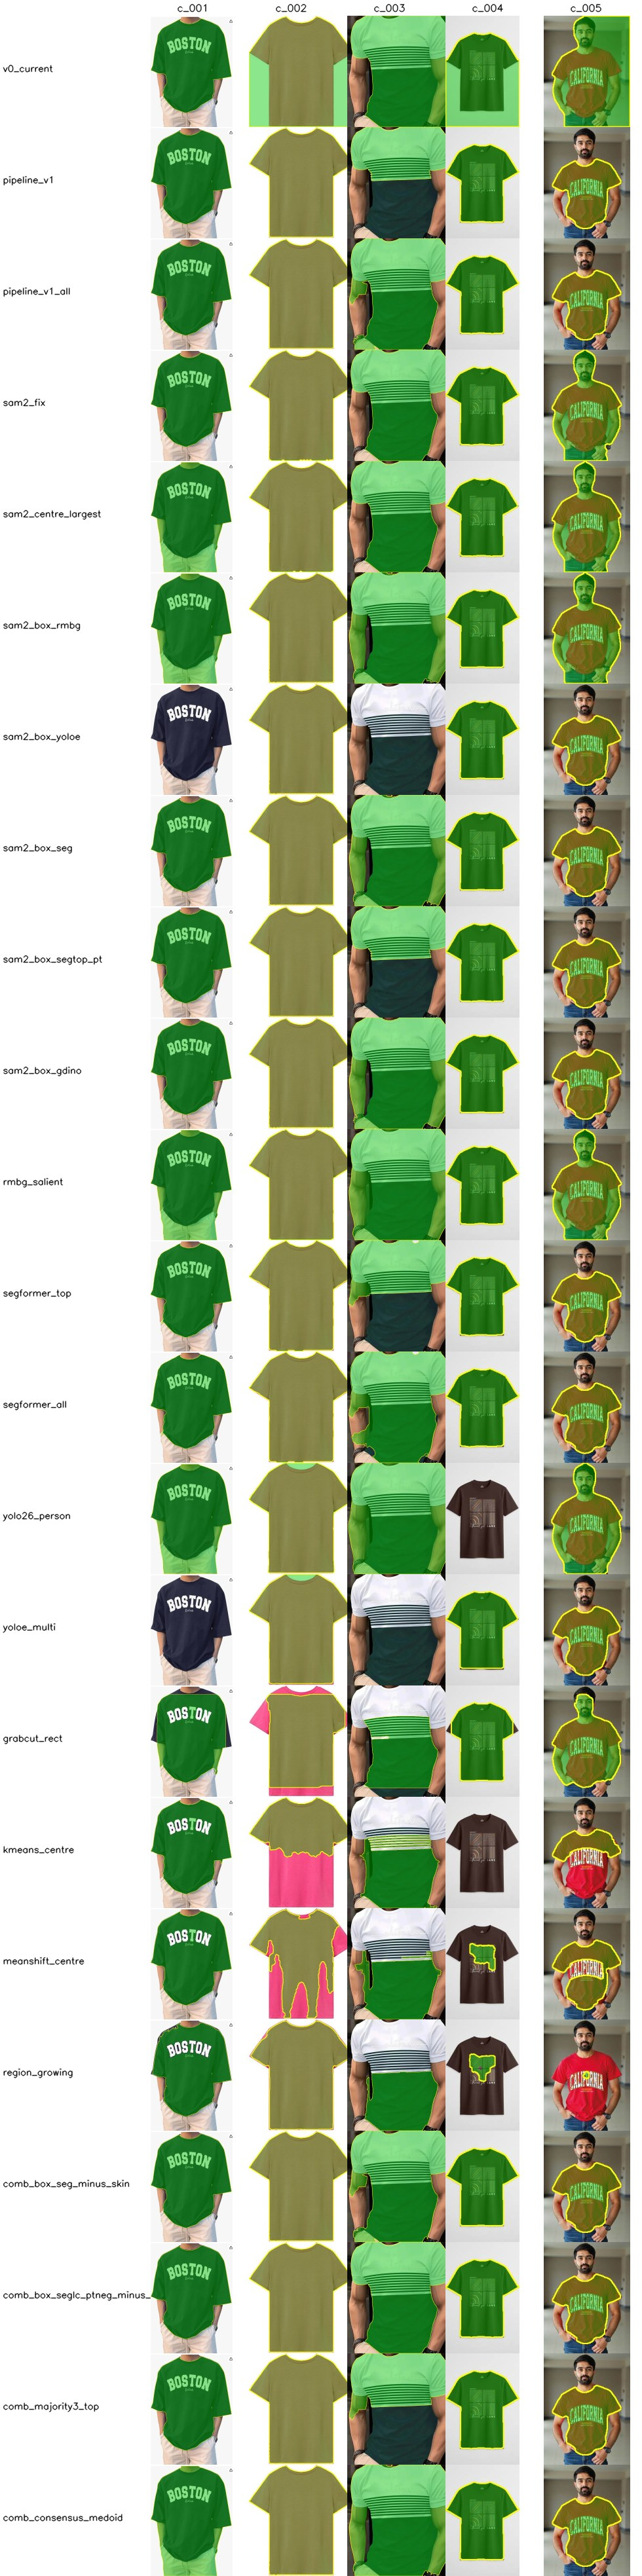
\includegraphics[width=\textwidth,height=0.42\textheight,keepaspectratio]{p01_contact_sheet_selected.jpg}
\caption{Segmentation methods (rows) on the five product photos (columns): classical, zero-shot and combined methods.}
\label{fig:p01sheet}
\end{figure*}

\subsection{Filtering, colour and designs}
Among 117 smoothing/edge-detector combinations, a bilateral filter followed by Laplacian zero crossings gave the best print-edge F1 (0.734 vs.\ 0.630 for v0) while lowering false edges on plain fabric from 1.02\,\% to 0.65\,\% (Fig.~\ref{fig:edges}); global enhancement (histogram equalisation, CLAHE~\cite{zuiderveld1994}, Retinex~\cite{land1971}) shifted fabric colours and was not used before colour extraction. The colour stage raised colour-name accuracy on 266 product photos from 0.207 to 0.301 and recovers both fabric blocks of the colour-block top (Fig.~\ref{fig:colour}). For designs, the old FFT test fired on 100\,\% of plain and printed Fashionpedia garments; the rebuilt test fires on 8.3\,\% of plain and 40.9\,\% of printed ones. On the five photos the design score rose from 0.215 (v0 on the new masks) to 0.774 with the combined proposals and to 0.904 with SigLIP~2 relabelling (Fig.~\ref{fig:designs}). Gabor and wavelet texture segmentation responded to folds as strongly as to prints.

\begin{figure}[t]
\centering
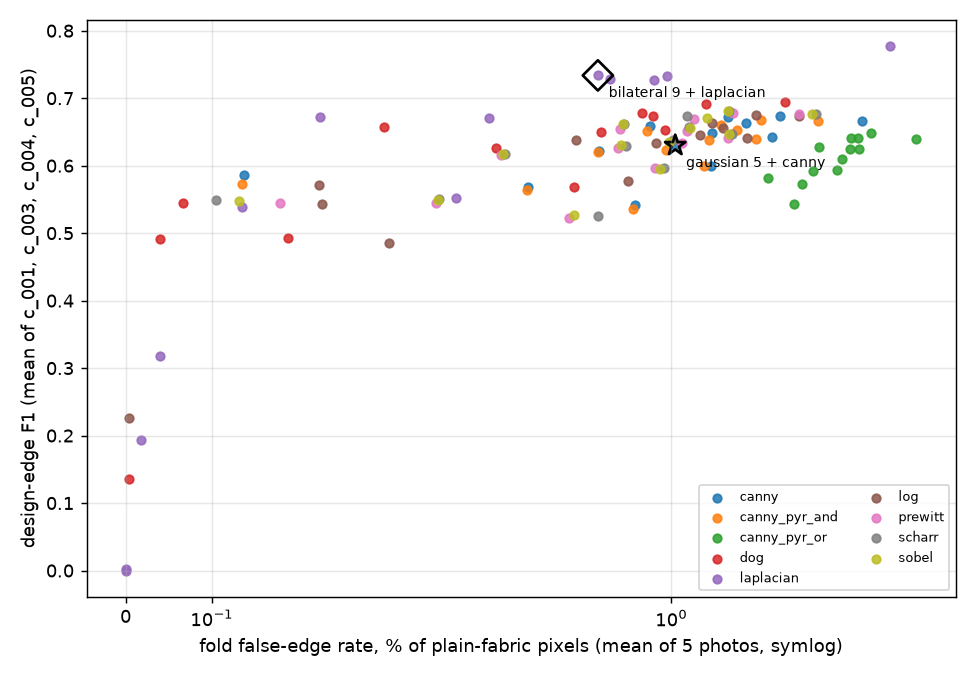
\includegraphics[width=\columnwidth,height=0.25\textheight,keepaspectratio]{p03_fig4_f1_vs_false_edges.png}
\caption{Print-edge F1 against false edges on plain fabric for all smoothing filter and edge detector combinations.}
\label{fig:edges}
\end{figure}

\begin{figure}[t]
\centering
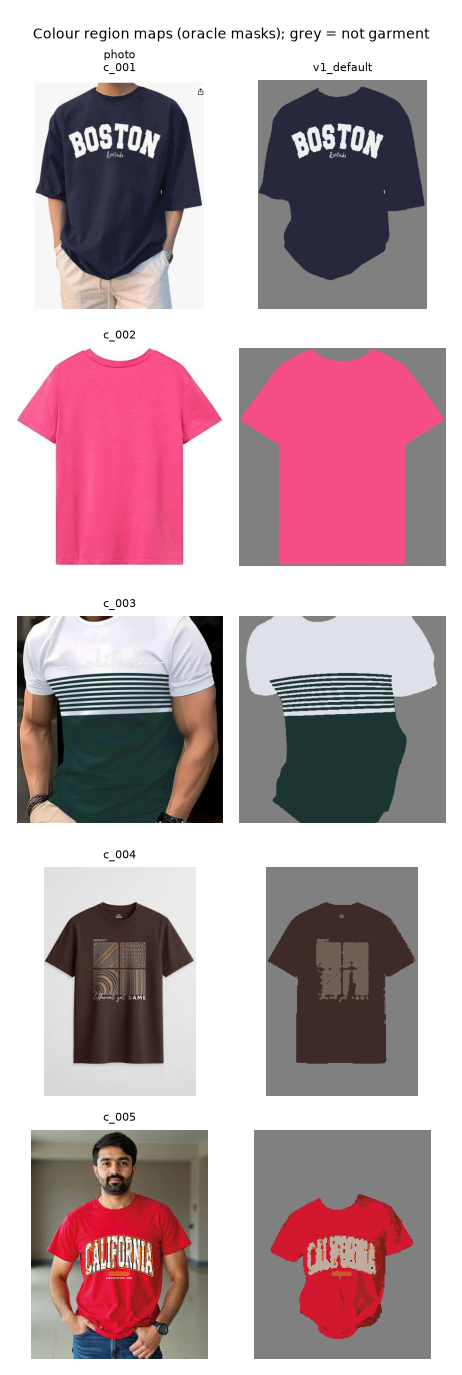
\includegraphics[width=\columnwidth,height=0.25\textheight,keepaspectratio]{p04_region_maps_oracle.png}
\caption{Colour region maps from the compared clustering methods; the colour-block top keeps both fabric blocks.}
\label{fig:colour}
\end{figure}

\begin{figure*}[t]
\centering
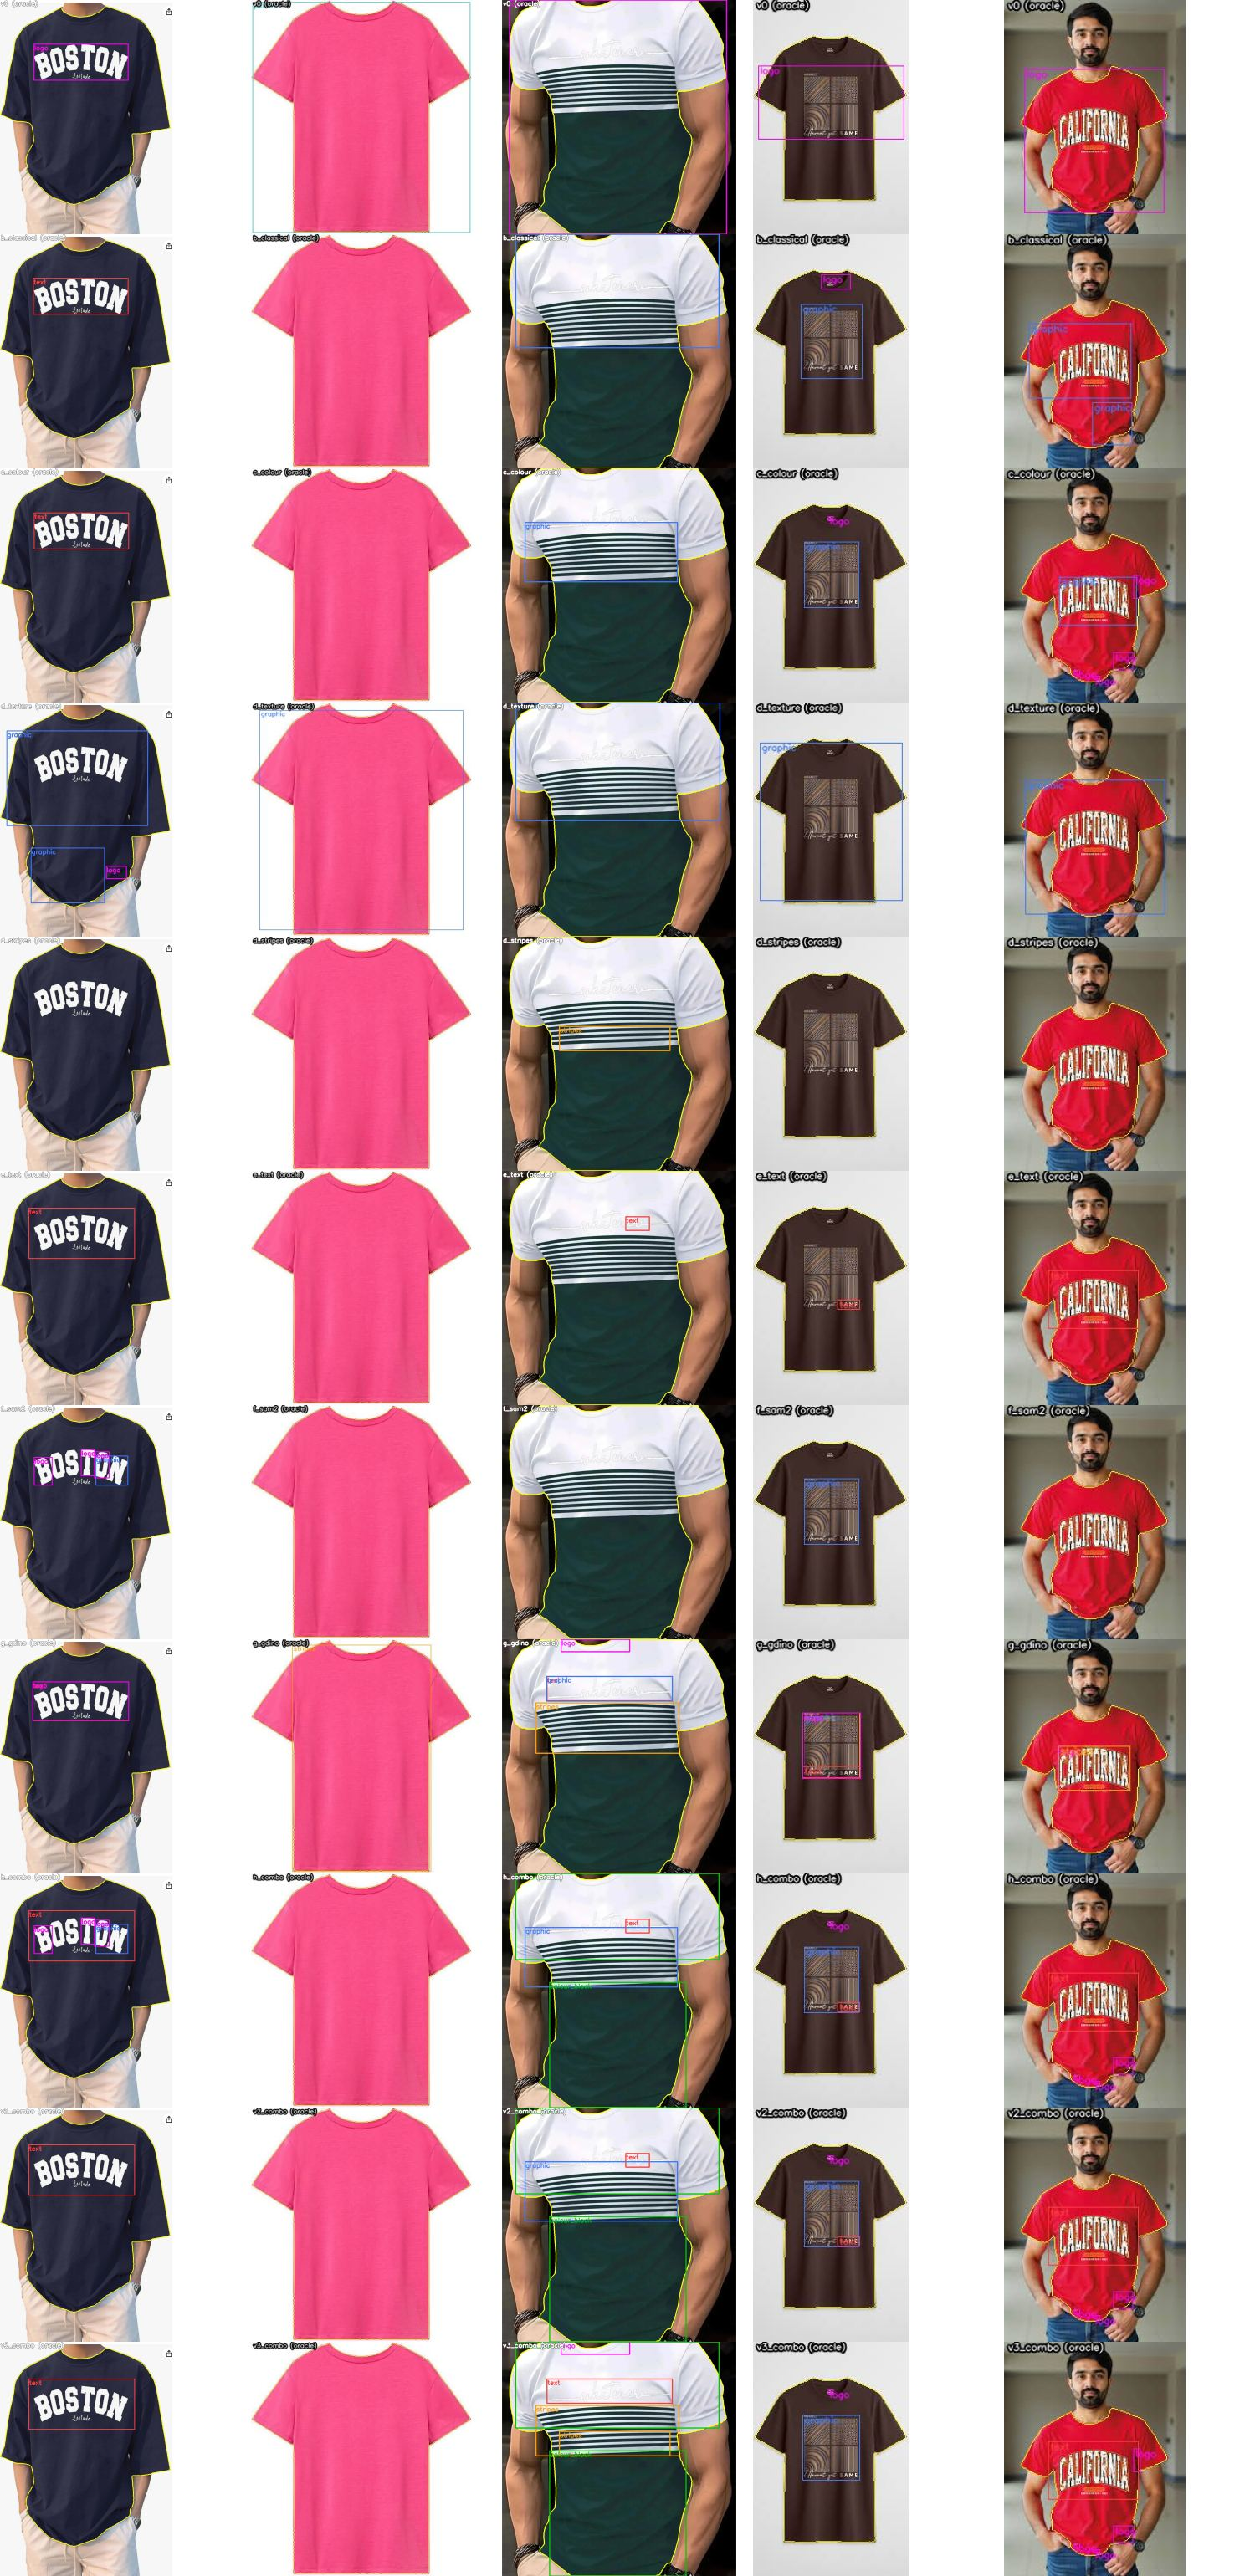
\includegraphics[width=\textwidth,height=0.42\textheight,keepaspectratio]{p05_contact_sheet_oracle_masks.jpg}
\caption{Two-level outlining: design regions found by each method (rows) inside the garment on the five photos (columns).}
\label{fig:designs}
\end{figure*}

\subsection{Views, attributes, shape and panel textures}
The trained view classifier with the joint decision picks the correct front in 85.4\,\% of shuffled In-shop photo sets, against 61.7\,\% for taking the first photo; back recall is 0.98, and a photo of another garment is flagged 96.7\,\% of the time (Fig.~\ref{fig:views}). In a demonstration on two shuffled, renamed photo sets, front and back were both assigned correctly. The trained sleeve-length classifier reaches macro-F1 0.843 (three classes); pattern (0.518) and neckline (0.487) are limited by few training examples. On 327 VITON-HD tops the measured hem/chest ratio has median 1.16, against the fixed 0.93 of the parametric block, which motivates reading shape from photos. Per-panel thin-plate-spline maps raise body-panel silhouette IoU from 0.64--0.87 to 0.87--0.98 on nine photos (Fig.~\ref{fig:panels}).

\begin{figure}[t]
\centering
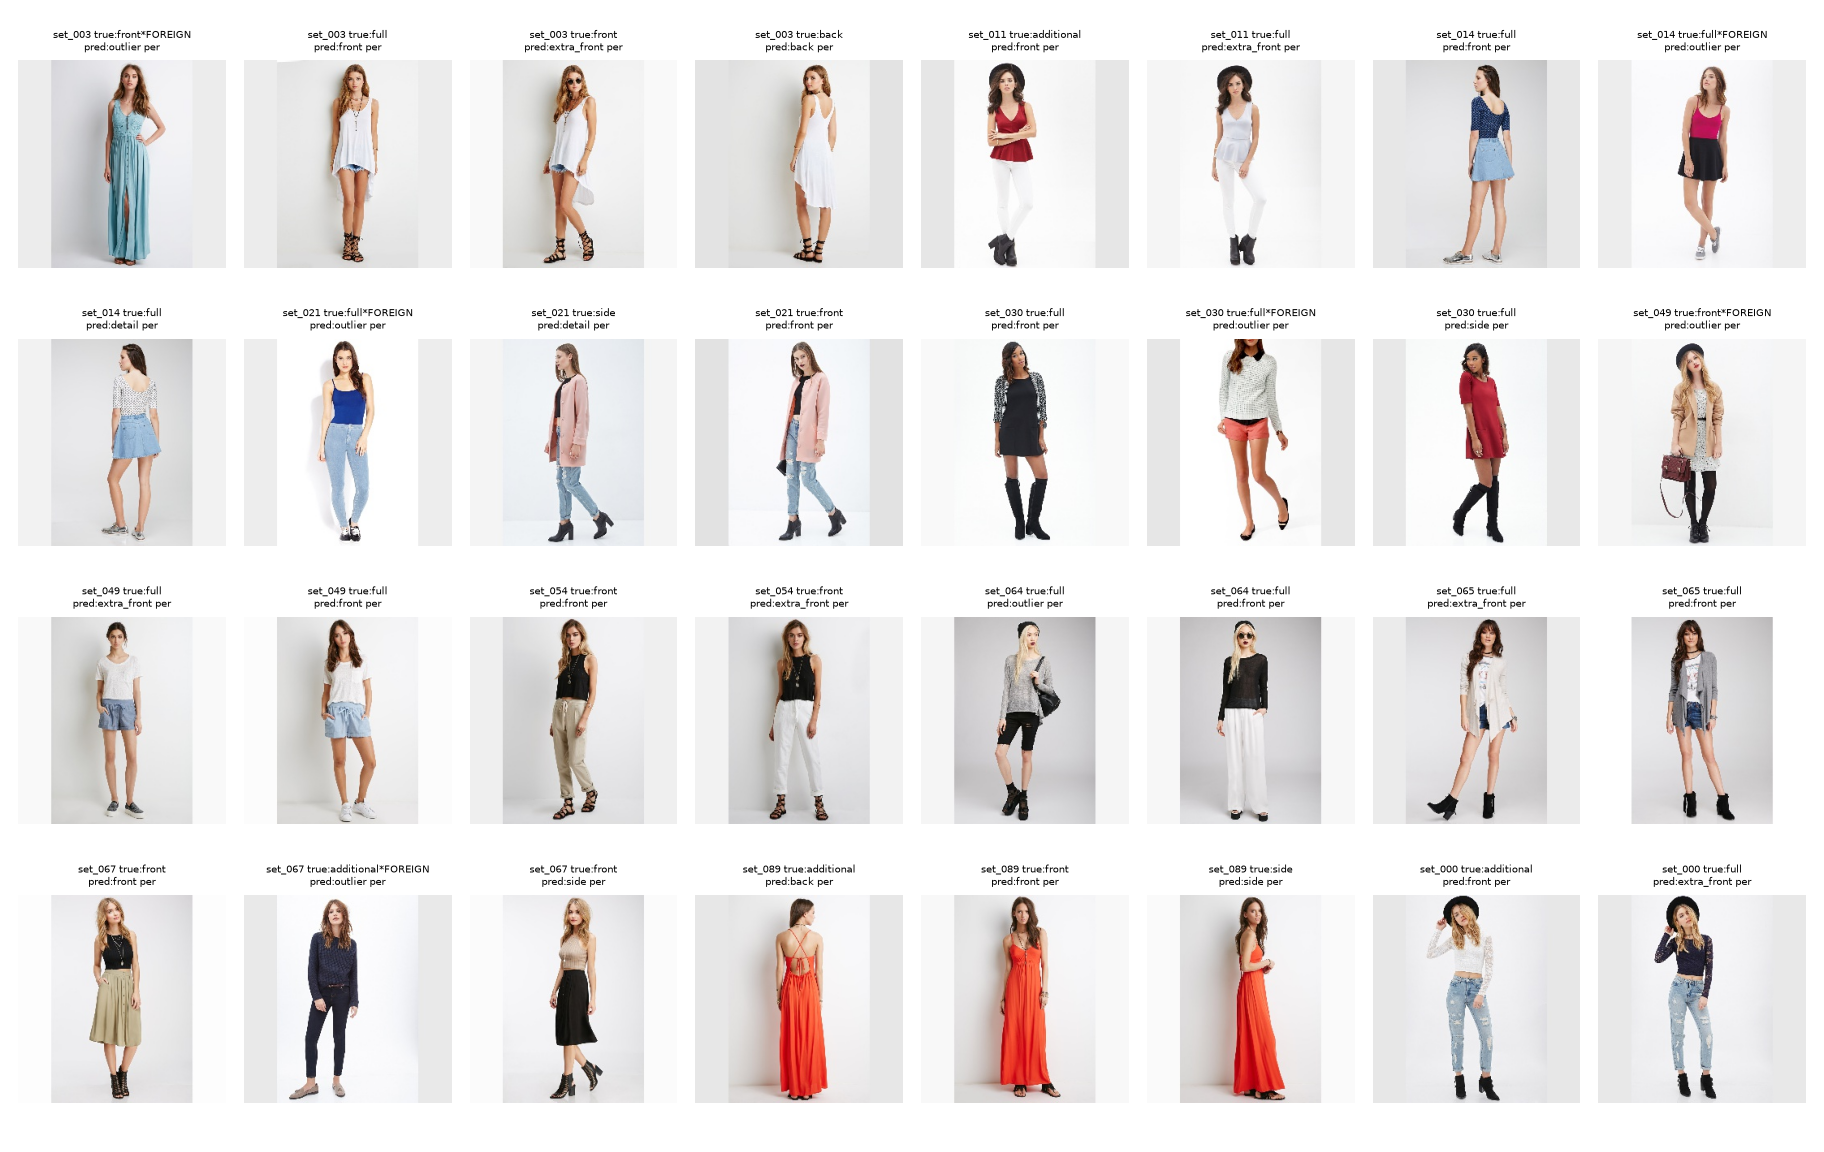
\includegraphics[width=\columnwidth,height=0.3\textheight,keepaspectratio]{p16_examples_testsets.png}
\caption{Shuffled photo sets with the front and back chosen by the trained classifier and the joint decision.}
\label{fig:views}
\end{figure}

\begin{figure}[t]
\centering
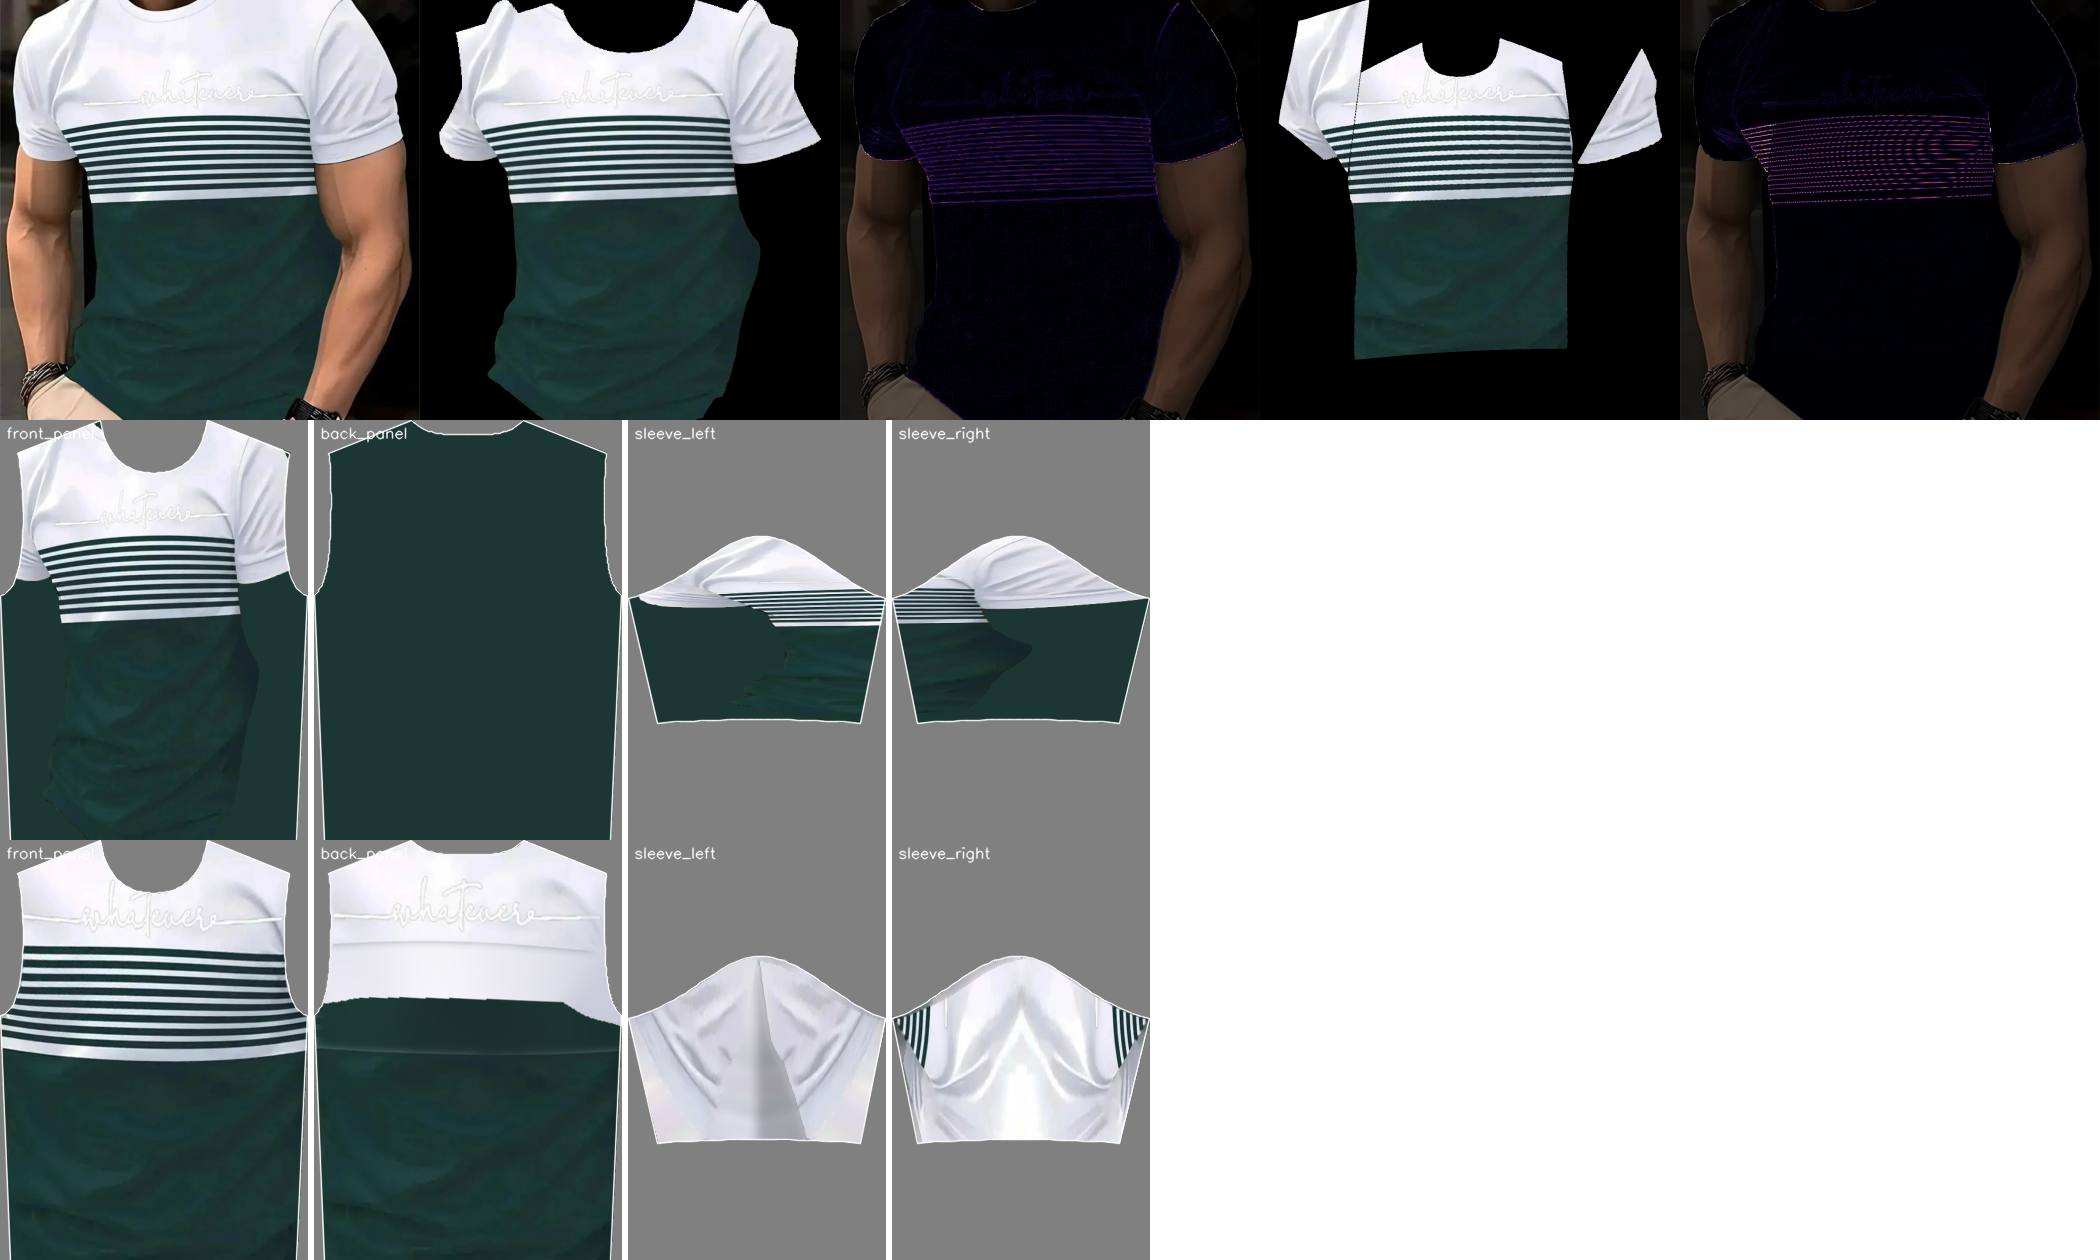
\includegraphics[width=\columnwidth,height=0.25\textheight,keepaspectratio]{p19_panel_maps_c_003.jpg}
\caption{Panel textures for the colour-block top: v0 box warp against the per-panel thin-plate-spline maps.}
\label{fig:panels}
\end{figure}

\section{Discussion and Limitations}
The largest single gain came from the prompt, not the model: the same SAM~2 performs far better when a clothes parser tells it where the garment is. Simple scene reasoning on top of model outputs (is a head visible?) fixed the colour-block failure where every confidence-based rule failed, because the parser was 96\,\% confident in its wrong ``skirt'' label. Classical methods remain useful as components (bilateral filtering, Hough stripes, convexity defects, thin-plate splines) but not as stand-alone segmenters or texture classifiers.

The limitations are: five own photos with approximate references by one annotator, four of them started from SAM~2 candidates; design thresholds tuned while looking at these photos; the head rule rests on one real torso-crop example and has a small margin (0.3\,\% against 1.2\,\%); the fine-tuned YOLO was tested in-domain; view training photos are all on-model; shape from worn garments is unreliable; and the 3D drape in the simulator was not evaluated. The judge of the blind ranking also made the references.

\section{Conclusion}
Rebuilding the photo-reading stage with validated metrics and a stage-by-stage comparison of classical, zero-shot and trained methods raised the end-to-end score on real product photos from 0.407 to 0.960 and the public garment IoU from 0.756 to 0.892. The pipeline now accepts several unlabelled photos, never reduces a garment to one colour, and outlines and types every design region. Future work will add the user's own photos with a reference sheet for metric scale (homography), more training data for small text and multi-part prints, and evaluation of the draped 3D result.

\section*{Code Availability}
The implementation, scripts to reproduce every experiment, and all result tables are available at: \url{https://github.com/saumy-github/mirra-mvp}.

\begin{thebibliography}{99}

\bibitem{luo2026survey}
Luo, Qu, Zhao, Zhang, and Yang, ``Deep learning for 3D fashion design: A survey from a sewing-pattern-driven perspective,'' \emph{IEEE Trans. Circuits Syst. Video Technol.}, vol.~36, no.~4, 2026, doi: 10.1109/TCSVT.2025.3637565.

\bibitem{lyu2026review}
Lyu, Wang, Ye, Sun, and Chao, ``Body data-driven garment pattern construction in digital fashion innovations: A review,'' \emph{Textile Res. J.}, vol.~96, no.~11--12, pp.~1299--1335, 2026, doi: 10.1177/00405175251352800.

\bibitem{cannavo2024pipeline}
A.~Cannav\`{o}, Offre, and F.~Lamberti, ``A semiautomated pipeline for the creation of virtual fitting room experiences,'' \emph{IEEE Comput. Graph. Appl.}, 2024, doi: 10.1109/MCG.2024.3521716.

\bibitem{nikolaev2026quantfit}
Nikolaev, Roman, and Makarov, ``QuantFit-VTON: Measurement-conditioned diffusion model for predictable garment fit,'' \emph{IEEE Access}, 2026, doi: 10.1109/ACCESS.2026.3668411.

\bibitem{kim2025capvton}
Kim, Lee, Lee, and Lee, ``Clothing-agnostic pre-inpainting virtual try-on,'' \emph{Electronics}, vol.~14, no.~23, p.~4710, 2025.

\bibitem{ravi2024sam2}
N.~Ravi \emph{et al.}, ``SAM 2: Segment anything in images and videos,'' arXiv:2408.00714, 2024.

\bibitem{xie2021segformer}
E.~Xie, W.~Wang, Z.~Yu, A.~Anandkumar, J.~M.~Alvarez, and P.~Luo, ``SegFormer: Simple and efficient design for semantic segmentation with transformers,'' in \emph{Proc. NeurIPS}, 2021.

\bibitem{liu2024groundingdino}
S.~Liu \emph{et al.}, ``Grounding DINO: Marrying DINO with grounded pre-training for open-set object detection,'' in \emph{Proc. ECCV}, 2024.

\bibitem{ultralytics}
Ultralytics, ``Ultralytics YOLO (YOLO11, YOLO26, YOLOE),'' software, version 8.4.215, accessed Nov. 2026. [Online]. Available: \url{https://github.com/ultralytics/ultralytics}

\bibitem{rother2004grabcut}
C.~Rother, V.~Kolmogorov, and A.~Blake, ``GrabCut: Interactive foreground extraction using iterated graph cuts,'' \emph{ACM Trans. Graph.}, vol.~23, no.~3, pp.~309--314, 2004.

\bibitem{comaniciu2002meanshift}
D.~Comaniciu and P.~Meer, ``Mean shift: A robust approach toward feature space analysis,'' \emph{IEEE Trans. Pattern Anal. Mach. Intell.}, vol.~24, no.~5, pp.~603--619, 2002.

\bibitem{radford2021clip}
A.~Radford \emph{et al.}, ``Learning transferable visual models from natural language supervision,'' in \emph{Proc. ICML}, 2021.

\bibitem{tschannen2025siglip2}
M.~Tschannen \emph{et al.}, ``SigLIP 2: Multilingual vision-language encoders with improved semantic understanding, localization, and dense features,'' arXiv:2502.14786, 2025.

\bibitem{marqo2024fashionsiglip}
Marqo, ``Marqo-FashionSigLIP,'' model card, 2024. [Online]. Available: \url{https://huggingface.co/Marqo/marqo-fashionSigLIP}

\bibitem{jia2020fashionpedia}
M.~Jia \emph{et al.}, ``Fashionpedia: Ontology, segmentation, and an attribute localization dataset,'' in \emph{Proc. ECCV}, 2020.

\bibitem{choi2021vitonhd}
S.~Choi, S.~Park, M.~Lee, and J.~Choo, ``VITON-HD: High-resolution virtual try-on via misalignment-aware normalization,'' in \emph{Proc. CVPR}, 2021.

\bibitem{liu2016deepfashion}
Z.~Liu, P.~Luo, S.~Qiu, X.~Wang, and X.~Tang, ``DeepFashion: Powering robust clothes recognition and retrieval with rich annotations,'' in \emph{Proc. CVPR}, 2016.

\bibitem{aggarwal2019fpi}
P.~Aggarwal, ``Fashion product images (small),'' Kaggle dataset, 2019.

\bibitem{baek2019craft}
Y.~Baek, B.~Lee, D.~Han, S.~Yun, and H.~Lee, ``Character region awareness for text detection,'' in \emph{Proc. CVPR}, 2019.

\bibitem{mohammedkhan2025review}
Mohammedkhan, Fleuren, G\"{u}ven, and Postma, ``Inferring body measurements from 2D images: A comprehensive review,'' \emph{J. Imaging}, 2025, doi: 10.3390/jimaging11060205.

\bibitem{fisher1936lda}
R.~A.~Fisher, ``The use of multiple measurements in taxonomic problems,'' \emph{Ann. Eugenics}, vol.~7, no.~2, pp.~179--188, 1936.

\bibitem{douglas1973}
D.~H.~Douglas and T.~K.~Peucker, ``Algorithms for the reduction of the number of points required to represent a digitized line or its caricature,'' \emph{Cartographica}, vol.~10, no.~2, pp.~112--122, 1973.

\bibitem{sharma2005ciede2000}
G.~Sharma, W.~Wu, and E.~N.~Dalal, ``The CIEDE2000 color-difference formula: Implementation notes, supplementary test data, and mathematical observations,'' \emph{Color Res. Appl.}, vol.~30, no.~1, pp.~21--30, 2005.

\bibitem{kaufman1990}
L.~Kaufman and P.~J.~Rousseeuw, \emph{Finding Groups in Data: An Introduction to Cluster Analysis}. New York, NY, USA: Wiley, 1990.

\bibitem{duda1972hough}
R.~O.~Duda and P.~E.~Hart, ``Use of the Hough transformation to detect lines and curves in pictures,'' \emph{Commun. ACM}, vol.~15, no.~1, pp.~11--15, 1972.

\bibitem{jain1991gabor}
A.~K.~Jain and F.~Farrokhnia, ``Unsupervised texture segmentation using Gabor filters,'' \emph{Pattern Recognit.}, vol.~24, no.~12, pp.~1167--1186, 1991.

\bibitem{mallat1989}
S.~G.~Mallat, ``A theory for multiresolution signal decomposition: The wavelet representation,'' \emph{IEEE Trans. Pattern Anal. Mach. Intell.}, vol.~11, no.~7, pp.~674--693, 1989.

\bibitem{canny1986}
J.~Canny, ``A computational approach to edge detection,'' \emph{IEEE Trans. Pattern Anal. Mach. Intell.}, vol.~PAMI-8, no.~6, pp.~679--698, 1986.

\bibitem{harris1988}
C.~Harris and M.~Stephens, ``A combined corner and edge detector,'' in \emph{Proc. Alvey Vision Conf.}, 1988, pp.~147--151.

\bibitem{shi1994}
J.~Shi and C.~Tomasi, ``Good features to track,'' in \emph{Proc. CVPR}, 1994, pp.~593--600.

\bibitem{rublee2011orb}
E.~Rublee, V.~Rabaud, K.~Konolige, and G.~Bradski, ``ORB: An efficient alternative to SIFT or SURF,'' in \emph{Proc. ICCV}, 2011, pp.~2564--2571.

\bibitem{lowe2004sift}
D.~G.~Lowe, ``Distinctive image features from scale-invariant keypoints,'' \emph{Int. J. Comput. Vis.}, vol.~60, no.~2, pp.~91--110, 2004.

\bibitem{bookstein1989tps}
F.~L.~Bookstein, ``Principal warps: Thin-plate splines and the decomposition of deformations,'' \emph{IEEE Trans. Pattern Anal. Mach. Intell.}, vol.~11, no.~6, pp.~567--585, 1989.

\bibitem{kendall1938}
M.~G.~Kendall, ``A new measure of rank correlation,'' \emph{Biometrika}, vol.~30, no.~1--2, pp.~81--93, 1938.

\bibitem{zuiderveld1994}
K.~Zuiderveld, ``Contrast limited adaptive histogram equalization,'' in \emph{Graphics Gems IV}, P.~S.~Heckbert, Ed. San Diego, CA, USA: Academic Press, 1994, pp.~474--485.

\bibitem{land1971}
E.~H.~Land and J.~J.~McCann, ``Lightness and Retinex theory,'' \emph{J. Opt. Soc. Amer.}, vol.~61, no.~1, pp.~1--11, 1971.

\end{thebibliography}

\end{document}
